% ======================================================================
%  Rapport scientifique - Sujet 5 : Vision Foundation Models and SSL
%  Compilation : pdflatex rapport && bibtex rapport && pdflatex rapport x2
% ======================================================================
\documentclass[11pt,a4paper]{article}
\usepackage[T1]{fontenc}
\usepackage[utf8]{inputenc}
\usepackage[french]{babel}
\usepackage{lmodern}
\usepackage[a4paper,margin=2.2cm,top=2cm,bottom=2.2cm]{geometry}
\usepackage{amsmath,amssymb,bm,pifont}
\usepackage{booktabs,array,tabularx,multirow}
\usepackage{graphicx}
\usepackage{caption,subcaption}
\usepackage{xcolor}
\usepackage{tikz}
\usetikzlibrary{arrows.meta,positioning,calc,decorations.pathreplacing}
\usepackage[numbers,sort&compress]{natbib}
\usepackage[hidelinks]{hyperref}
\usepackage{fancyhdr}
\usepackage{titlesec}
\usepackage{enumitem}
\graphicspath{{../figures/}}
% Couleurs et styles TikZ partagés (présentation + rapport)
\definecolor{bleuE}{HTML}{1F5F8B}
\definecolor{bleuclair}{HTML}{E6F0F7}
\definecolor{orangeE}{HTML}{E07B1A}
\definecolor{orangeclair}{HTML}{FCEBD9}
\definecolor{vertE}{HTML}{2E8B57}
\definecolor{vertclair}{HTML}{E2F2E8}
\definecolor{violetE}{HTML}{6250D6}
\definecolor{violetclair}{HTML}{ECEAFB}
\definecolor{grisE}{HTML}{5F5F5F}
\definecolor{grisclair}{HTML}{F2F2F2}
\definecolor{rougeE}{HTML}{C0392B}

\tikzset{
  box/.style={draw=bleuE, fill=bleuclair, rounded corners=3pt, align=center, font=\small,
              inner sep=3pt, minimum height=8mm, line width=0.7pt},
  obox/.style={box, draw=orangeE, fill=orangeclair},
  gbox/.style={box, draw=vertE, fill=vertclair},
  vbox/.style={box, draw=violetE, fill=violetclair},
  nbox/.style={box, draw=grisE, fill=grisclair},
  arr/.style={-{Stealth[length=2.2mm]}, line width=0.8pt, draw=grisE},
  darr/.style={arr, dashed},
  lbl/.style={font=\scriptsize, text=grisE, align=center},
  tok/.style={draw=white, line width=0.5pt, minimum size=2.6mm, inner sep=0pt},
}

\IfFileExists{../figures/results.tex}{% Généré automatiquement par notebook/demo_dinov2.ipynb -- ne pas éditer à la main
\providecommand{\RnTrain}{1\,840}
\providecommand{\RnTest}{1\,840}
\providecommand{\RKnnDinoS}{92{,}1\,\%}
\providecommand{\RLinDinoS}{94{,}9\,\%}
\providecommand{\RKnnClsDinoS}{92{,}1\,\%}
\providecommand{\RKnnMeanDinoS}{78{,}4\,\%}
\providecommand{\RPoneDinoS}{92{,}0\,\%}
\providecommand{\RPfiveDinoS}{88{,}8\,\%}
\providecommand{\RPtenDinoS}{85{,}8\,\%}
\providecommand{\RSoneDinoS}{70{,}9\,\%}
\providecommand{\RStwoDinoS}{80{,}8\,\%}
\providecommand{\RSfiveDinoS}{88{,}6\,\%}
\providecommand{\RStenDinoS}{91{,}5\,\%}
\providecommand{\RStwentyDinoS}{93{,}0\,\%}
\providecommand{\RSallDinoS}{94{,}9\,\%}
\providecommand{\RSilDinoS}{0{,}217}
\providecommand{\RIouDinoS}{66{,}9\,\%}
\providecommand{\RParamsDinoS}{22\,M}
\providecommand{\RIpsDinoS}{735}
\providecommand{\RVramDinoS}{145\,Mo}
\providecommand{\RExtDinoS}{23\,s}
\providecommand{\RPoolDinoS}{[CLS]}
\providecommand{\RCDinoS}{0.1}
\providecommand{\RKnnDinoB}{94{,}0\,\%}
\providecommand{\RLinDinoB}{96{,}4\,\%}
\providecommand{\RKnnClsDinoB}{94{,}0\,\%}
\providecommand{\RKnnMeanDinoB}{79{,}9\,\%}
\providecommand{\RPoneDinoB}{93{,}5\,\%}
\providecommand{\RPfiveDinoB}{90{,}9\,\%}
\providecommand{\RPtenDinoB}{89{,}0\,\%}
\providecommand{\RSoneDinoB}{78{,}6\,\%}
\providecommand{\RStwoDinoB}{86{,}1\,\%}
\providecommand{\RSfiveDinoB}{91{,}2\,\%}
\providecommand{\RStenDinoB}{93{,}6\,\%}
\providecommand{\RStwentyDinoB}{94{,}7\,\%}
\providecommand{\RSallDinoB}{96{,}4\,\%}
\providecommand{\RSilDinoB}{0{,}283}
\providecommand{\RIouDinoB}{66{,}7\,\%}
\providecommand{\RParamsDinoB}{87\,M}
\providecommand{\RIpsDinoB}{236}
\providecommand{\RVramDinoB}{358\,Mo}
\providecommand{\RExtDinoB}{36\,s}
\providecommand{\RPoolDinoB}{[CLS]}
\providecommand{\RCDinoB}{0.1}
\providecommand{\RKnnMae}{21{,}0\,\%}
\providecommand{\RLinMae}{83{,}8\,\%}
\providecommand{\RKnnClsMae}{21{,}0\,\%}
\providecommand{\RKnnMeanMae}{19{,}6\,\%}
\providecommand{\RPoneMae}{22{,}8\,\%}
\providecommand{\RPfiveMae}{13{,}8\,\%}
\providecommand{\RPtenMae}{10{,}6\,\%}
\providecommand{\RSoneMae}{18{,}4\,\%}
\providecommand{\RStwoMae}{27{,}5\,\%}
\providecommand{\RSfiveMae}{47{,}9\,\%}
\providecommand{\RStenMae}{62{,}9\,\%}
\providecommand{\RStwentyMae}{74{,}1\,\%}
\providecommand{\RSallMae}{83{,}8\,\%}
\providecommand{\RSilMae}{-0{,}291}
\providecommand{\RIouMae}{48{,}8\,\%}
\providecommand{\RParamsMae}{86\,M}
\providecommand{\RIpsMae}{287}
\providecommand{\RVramMae}{298\,Mo}
\providecommand{\RExtMae}{30\,s}
\providecommand{\RPoolMae}{[CLS]}
\providecommand{\RCMae}{0.1}
\providecommand{\RKnnDeit}{92{,}3\,\%}
\providecommand{\RLinDeit}{94{,}4\,\%}
\providecommand{\RKnnClsDeit}{92{,}3\,\%}
\providecommand{\RKnnMeanDeit}{86{,}2\,\%}
\providecommand{\RPoneDeit}{91{,}8\,\%}
\providecommand{\RPfiveDeit}{88{,}5\,\%}
\providecommand{\RPtenDeit}{86{,}7\,\%}
\providecommand{\RSoneDeit}{74{,}6\,\%}
\providecommand{\RStwoDeit}{83{,}3\,\%}
\providecommand{\RSfiveDeit}{89{,}2\,\%}
\providecommand{\RStenDeit}{91{,}2\,\%}
\providecommand{\RStwentyDeit}{92{,}5\,\%}
\providecommand{\RSallDeit}{94{,}4\,\%}
\providecommand{\RSilDeit}{0{,}311}
\providecommand{\RIouDeit}{63{,}3\,\%}
\providecommand{\RParamsDeit}{22\,M}
\providecommand{\RIpsDeit}{726}
\providecommand{\RVramDeit}{115\,Mo}
\providecommand{\RExtDeit}{25\,s}
\providecommand{\RPoolDeit}{[CLS]}
\providecommand{\RCDeit}{1}
\providecommand{\RIouCenter}{49{,}3\,\%}
\providecommand{\RbestModel}{DINOv2-B/14}
\providecommand{\RconfOne}{American Pit Bull Terrier $\to$ Staffordshire Bull Terrier (7)}
\providecommand{\RconfTwo}{Staffordshire Bull Terrier $\to$ American Bulldog (5)}
\providecommand{\RconfThree}{Ragdoll $\to$ Birman (5)}
\providecommand{\RsearchTrue}{Siamese}
\providecommand{\RsearchCrop}{Siamese}
\providecommand{\RsearchSketch}{Russian Blue}
\providecommand{\RsearchCropConf}{100{,}0\,\%}
\providecommand{\RsearchSketchConf}{67{,}5\,\%}
}{}

\setlist{itemsep=1pt,topsep=3pt}
\newcolumntype{L}{>{\raggedright\arraybackslash}X}
\captionsetup{font=small,labelfont=bf}
\titleformat{\section}{\large\bfseries\color{bleuE}}{\thesection.}{0.5em}{}
\titleformat{\subsection}{\normalsize\bfseries\color{bleuE}}{\thesubsection}{0.5em}{}
\titlespacing*{\section}{0pt}{10pt}{4pt}
\titlespacing*{\subsection}{0pt}{7pt}{3pt}
\pagestyle{fancy}\fancyhf{}
\renewcommand{\headrulewidth}{0.4pt}
\fancyhead[L]{\small\color{grisE}Sujet 5 -- Vision Foundation Models \& Self-Supervised Learning}
\fancyhead[R]{\small\color{grisE}ENSAM Meknès}
\fancyfoot[C]{\small\thepage}

\begin{document}

% ---------------------------------------------------------------- en-tête
\thispagestyle{empty}
\noindent\begin{minipage}[c]{0.42\textwidth}
  
\includegraphics[height=1.35cm]{logos_umi_ensam.pdf}
\end{minipage}\hfill
\begin{minipage}[c]{0.56\textwidth}\raggedleft\small
  \textbf{Université Moulay Ismail}\\École Nationale Supérieure d'Arts et Métiers -- Meknès\\Cours : LLM, LVM \& GenAI -- Fondations et Applications
\end{minipage}
\vspace{4mm}
{\color{bleuE}\rule{\textwidth}{1.2pt}}
\begin{center}
  {\small\color{grisE}RAPPORT SCIENTIFIQUE -- EXPOSÉS LARGE VISION MODELS -- SUJET 5}\\[2mm]
  {\LARGE\bfseries\color{bleuE} Vision Foundation Models and Self-Supervised Learning}\\[2mm]
  {\large Apprendre des représentations visuelles réutilisables sans étiquettes :\\ du contrastif à MAE et DINOv2}\\[4mm]
  \begin{tabular}{c@{\hspace{1.2cm}}c}
    \textbf{NANKOULI} Marc Thierry & \textbf{DIALLO} Souleymane\\
    \textbf{HINIMDOU} Morsia Guitdam & \textbf{CHAIBOU SAIDOU} Abdoulaye
  \end{tabular}\\[2mm]
  Encadrant : \textbf{Pr. ELANSARI} \hspace{1cm} Novembre 2026
\end{center}
{\color{bleuE}\rule{\textwidth}{0.6pt}}

\begin{abstract}
\noindent Les \emph{Vision Foundation Models} (VFM) sont des encodeurs visuels pré-entraînés à grande échelle, puis réutilisés sur de nombreuses tâches avec peu de données annotées. Leur principal moteur est l'apprentissage auto-supervisé (\emph{Self-Supervised Learning}, SSL), qui tire la supervision des images elles-mêmes. Ce rapport présente les principes du SSL, détaille les deux grandes familles que sont l'apprentissage contrastif et le \emph{Masked Image Modeling}, puis étudie deux modèles de référence : les \emph{Masked Autoencoders} (MAE) et DINOv2. Nous évaluons ensuite expérimentalement la réutilisation de représentations \emph{gelées} sur Oxford-IIIT Pets (37 races). Sans aucun fine-tuning, DINOv2-B/14 atteint \RLinDinoB{} d'exactitude avec une simple sonde linéaire et \RKnnDinoB{} avec un k-NN, et \RSoneDinoB{} avec une seule image étiquetée par classe. À taille égale, DINOv2-S/14 (\RLinDinoS) fait jeu égal avec un ViT supervisé sur ImageNet (DeiT-S, \RLinDeit) sans avoir vu une seule étiquette. MAE, dont les features sont peu linéairement séparables, plafonne à \RLinMae{} et s'effondre en k-NN (\RKnnMae). Nous discutons enfin les performances, les limites et les coûts de ces approches.
\end{abstract}

% ======================================================================
\section{Introduction}
La vision par ordinateur a longtemps reposé sur l'apprentissage supervisé : un réseau est entraîné à prédire des étiquettes annotées à la main, comme les 14 millions d'images d'ImageNet. Cette approche a deux limites. Annoter coûte cher et demande parfois une expertise rare (imagerie médicale, inspection industrielle). Surtout, une étiquette est une information pauvre : un seul mot pour décrire une image riche en formes, textures, parties et contexte. Le web contient pourtant des milliards d'images non annotées.

L'apprentissage auto-supervisé apprend des représentations à partir de ces données brutes, en résolvant des \emph{tâches prétextes} dont la supervision est générée automatiquement. Associé au passage à l'échelle (données, modèles, calcul), il donne naissance aux \emph{Vision Foundation Models}, des encodeurs généralistes qu'on adapte ensuite à moindre coût. Ce rapport poursuit trois objectifs : (i) définir les VFM et les principes du SSL ; (ii) expliquer l'apprentissage contrastif et le \emph{Masked Image Modeling}, en détaillant MAE et DINOv2 ; (iii) mesurer expérimentalement la réutilisabilité des représentations obtenues, sur une tâche de recherche de similarité et de classification simple.

% ======================================================================
\section{État de l'art}
\subsection{Vision Foundation Models}
\citet{bommasani2021foundation} définissent un modèle de fondation comme un modèle entraîné sur des données larges, généralement par auto-supervision à grande échelle, et adaptable à un large éventail de tâches. En vision, ces modèles présentent cinq caractéristiques : l'\textbf{échelle} ($10^8$ à $10^9$ images, jusqu'à plusieurs milliards de paramètres) ; la \textbf{généralité} des représentations ; l'\textbf{adaptabilité} (k-NN, sonde linéaire, fine-tuning, adaptation paramétriquement efficace) ; l'\textbf{émergence} de capacités non enseignées (segmentation, correspondances) ; et l'\textbf{homogénéisation}, puisqu'un même backbone sert à de nombreuses tâches et leur transmet aussi ses défauts. La figure~\ref{fig:paradigme} résume ce paradigme.

\begin{figure}[ht]
  \centering
  \resizebox{0.92\textwidth}{!}{% Paradigme des Vision Foundation Models : pré-entraîner une fois, adapter partout
\begin{tikzpicture}
  \node[nbox, minimum width=31mm, minimum height=24mm] (data) at (0,0)
    {\textbf{Données massives}\\non étiquetées\\[3pt]{\scriptsize web, $10^8$ à $10^9$ images}};
  \node[box, minimum width=33mm, minimum height=26mm, line width=1.3pt] (vfm) at (5.9,0)
    {\textbf{Vision Foundation}\\\textbf{Model}\\[3pt]{\scriptsize encodeur ViT}\\{\scriptsize $10^7$ à $10^9$ paramètres}};
  \draw[arr] (data.east) -- node[lbl, above=1pt]{pré-entraînement\\\textbf{auto-supervisé}} node[lbl, below=1pt]{coûteux,\\une seule fois} (vfm.west);

  \node[gbox, minimum width=36mm, minimum height=6mm, anchor=west] (t1) at (10.0, 1.6) {Classification};
  \node[gbox, minimum width=36mm, minimum height=6mm, anchor=west] (t2) at (10.0, 0.8) {Recherche d'images};
  \node[gbox, minimum width=36mm, minimum height=6mm, anchor=west] (t3) at (10.0, 0.0) {Segmentation};
  \node[gbox, minimum width=36mm, minimum height=6mm, anchor=west] (t4) at (10.0,-0.8) {Estimation de profondeur};
  \node[gbox, minimum width=36mm, minimum height=6mm, anchor=west] (t5) at (10.0,-1.6) {Détection, suivi, \dots};
  \foreach \t in {t1,t2,t3,t4,t5} \draw[arr] (vfm.east) -- (\t.west);
  \node[lbl, above=1mm of t1] {adaptation légère, \textbf{peu de labels}};
\end{tikzpicture}
}
  \caption{Paradigme des VFM : un pré-entraînement auto-supervisé coûteux, réalisé une seule fois, puis une adaptation légère à de multiples tâches.}
  \label{fig:paradigme}
\end{figure}

On distingue trois manières de pré-entraîner un VFM : la supervision à grande échelle (ViT sur JFT-300M~\citep{dosovitskiy2021vit}) ; la supervision faible par le texte (CLIP, 400 M paires image-texte~\citep{radford2021clip}) ; et l'auto-supervision sur images seules, à laquelle ce rapport est consacré. Des modèles promptables comme SAM~\citep{kirillov2023sam} complètent ce paysage.

\subsection{Évolution de l'apprentissage auto-supervisé}
La figure~\ref{fig:timeline} retrace dix ans de SSL en vision. Les premières \emph{tâches prétextes} (prédire une rotation~\citep{gidaris2018rotation}, résoudre un puzzle~\citep{noroozi2016jigsaw}) produisaient des représentations trop spécialisées. À partir de 2018, la \emph{discrimination d'instances}~\citep{wu2018instdisc} et l'apprentissage contrastif (CPC~\citep{oord2018cpc}, MoCo~\citep{he2020moco}, SimCLR~\citep{chen2020simclr}) ont fortement réduit l'écart avec le supervisé. BYOL~\citep{grill2020byol} puis DINO~\citep{caron2021dino} ont montré qu'on pouvait se passer d'exemples négatifs grâce à l'auto-distillation, tandis que SwAV~\citep{caron2020swav} s'appuie sur un clustering en ligne. L'arrivée des Vision Transformers~\citep{dosovitskiy2021vit} a rendu possible le \emph{Masked Image Modeling} : BEiT~\citep{bao2022beit}, MAE~\citep{he2022mae}, SimMIM~\citep{xie2022simmim}, iBOT~\citep{zhou2022ibot}. Enfin, DINOv2~\citep{oquab2024dinov2} puis DINOv3~\citep{simeoni2025dinov3} combinent ces idées et les portent à grande échelle.

\begin{figure}[ht]
  \centering
  \resizebox{\textwidth}{!}{% Frise chronologique de l'apprentissage auto-supervisé en vision (année de publication)
\begin{tikzpicture}[
    ev/.style={rounded corners=2pt, minimum width=16mm, minimum height=4.6mm, inner sep=1pt,
               font=\scriptsize\bfseries, text=white, align=center},
    P/.style={ev, fill=grisE}, C/.style={ev, fill=bleuE}, D/.style={ev, fill=vertE},
    M/.style={ev, fill=orangeE}, X/.style={ev, fill=violetE}]
  \def\dx{1.78}
  \draw[line width=1.2pt, grisE, -{Stealth[length=2.5mm]}] (-0.6,0) -- (7*\dx+0.9,0);
  \foreach \y [count=\i from 0] in {2016,2018,2020,2021,2022,2023,2024,2025} {
    \fill[grisE] (\i*\dx,0) circle (1.4pt);
    \node[font=\sffamily\footnotesize\bfseries, text=grisE, below=1pt] at (\i*\dx,0) {\y};
  }
  % chaque année : pile d'événements (de bas en haut)
  \node[P] at (0*\dx,0.45) {Jigsaw};
  \node[P] at (1*\dx,0.45) {Rotation};
  \node[C] at (1*\dx,0.97) {InstDisc};
  \node[C] at (1*\dx,1.49) {CPC};
  \node[C] at (2*\dx,0.45) {MoCo};
  \node[C] at (2*\dx,0.97) {SimCLR};
  \node[D] at (2*\dx,1.49) {BYOL};
  \node[C] at (2*\dx,2.01) {SwAV};
  \node[D] at (3*\dx,0.45) {DINO};
  \node[C] at (3*\dx,0.97) {MoCo v3};
  \node[X] at (3*\dx,1.49) {CLIP};
  \node[X] at (3*\dx,2.01) {ViT};
  \node[M] at (4*\dx,0.45) {BEiT};
  \node[M] at (4*\dx,0.97) {MAE};
  \node[M] at (4*\dx,1.49) {SimMIM};
  \node[D] at (4*\dx,2.01) {iBOT};
  \node[D] at (5*\dx,0.45) {DINOv2};
  \node[X] at (5*\dx,0.97) {I-JEPA};
  \node[X] at (5*\dx,1.49) {SAM};
  \node[D] at (6*\dx,0.45) {Registers};
  \node[D] at (7*\dx,0.45) {DINOv3};
  % légende
  \begin{scope}[shift={(0,-0.95)}, every node/.style={font=\scriptsize, text=grisE, anchor=west}]
    \fill[grisE]    (0.0,0) rectangle +(0.25,0.25); \node at (0.3,0.12)  {Tâches prétextes};
    \fill[bleuE]    (2.75,0) rectangle +(0.25,0.25); \node at (3.05,0.12) {Contrastif};
    \fill[vertE]    (4.85,0) rectangle +(0.25,0.25); \node at (5.15,0.12) {Auto-distillation};
    \fill[orangeE]  (7.55,0) rectangle +(0.25,0.25); \node at (7.85,0.12) {Masquage (MIM)};
    \fill[violetE] (10.45,0) rectangle +(0.25,0.25); \node at (10.75,0.12) {Autres VFM / architectures};
  \end{scope}
\end{tikzpicture}
}
  \caption{Principales méthodes d'apprentissage auto-supervisé en vision, par année de publication et par famille.}
  \label{fig:timeline}
\end{figure}

% ======================================================================
\section{Fondements théoriques}
\subsection{Principe du Self-Supervised Learning}
Le SSL apprend un encodeur $f_\theta$ sur des images non étiquetées en minimisant la perte d'une tâche prétexte construite à partir des données. L'encodeur est ensuite transféré vers une tâche aval, gelé ou affiné, avec une tête légère entraînée sur peu de labels (figure~\ref{fig:ssl}). D'après la taxonomie de \citet{balestriero2023cookbook}, les méthodes modernes relèvent soit des architectures à \emph{plongement joint} (contrastif, auto-distillation, clustering), soit de la \emph{reconstruction} (masquage), soit de la \emph{prédiction dans l'espace latent} (I-JEPA~\citep{assran2023ijepa}).

\begin{figure}[ht]
  \centering
  \resizebox{0.8\textwidth}{!}{% Principe général du Self-Supervised Learning : pré-entraînement puis transfert
\begin{tikzpicture}
  % Étape 1
  \node[font=\small\bfseries, text=bleuE, anchor=west] at (-0.2,1.5) {\large\ding{172}\normalsize\ Pré-entraînement auto-supervisé (sans labels humains)};
  \node[nbox, minimum width=26mm] (u) at (1.1,0.4) {Images\\non étiquetées};
  \node[obox, minimum width=34mm] (p) at (5.0,0.4) {Tâche prétexte\\{\scriptsize la supervision est \textbf{tirée des données}}};
  \node[box, minimum width=24mm, line width=1.2pt] (f) at (8.9,0.4) {Encodeur $f_\theta$};
  \node[obox, minimum width=26mm] (l) at (12.4,0.4) {Perte\\{\scriptsize InfoNCE, MSE, CE\dots}};
  \draw[arr] (u) -- (p); \draw[arr] (p) -- (f); \draw[arr] (f) -- (l);
  \draw[darr, orangeE] (l.south) -- ++(0,-0.4) -| (9.7,0.0);
  \node[lbl, text=orangeE] at (11.2,-0.25) {rétro-propagation};
  \node[lbl, below=1pt of p.south, yshift=-3pt] {vues augmentées, patches masqués,\\rotation, ordre des pièces\dots};
  % séparateur
  \draw[grisE!60, dashed] (-0.2,-1.0) -- (13.9,-1.0);
  % Étape 2
  \node[font=\small\bfseries, text=vertE, anchor=west] at (-0.2,-1.4) {\large\ding{173}\normalsize\ Transfert vers une tâche aval};
  \node[gbox, minimum width=30mm] (d) at (5.0,-2.5) {Quelques images\\étiquetées};
  \node[box, minimum width=24mm, line width=1.2pt] (f2) at (8.9,-2.5) {Encodeur $f_\theta$\\{\scriptsize gelé ou affiné}};
  \node[gbox, minimum width=26mm] (h) at (12.4,-2.5) {Tête légère\\{\scriptsize $\rightarrow$ classe, masque\dots}};
  \draw[arr] (d) -- (f2); \draw[arr] (f2) -- (h);
  \draw[arr, bleuE, line width=1.3pt] (8.4,0.0) -- node[lbl, text=bleuE, fill=white, inner sep=1pt, pos=0.5]{\textbf{poids transférés}} (8.4,-2.1);
  \node[lbl, align=left, anchor=west] at (-0.2,-2.5) {peu de labels :\\de 1 à 100 images\\par classe};
\end{tikzpicture}
}
  \caption{Les deux temps du SSL : pré-entraînement sur une tâche prétexte, puis transfert vers une tâche aval.}
  \label{fig:ssl}
\end{figure}

\subsection{Apprentissage contrastif}
Deux vues $\tilde{x}_i$ et $\tilde{x}_j$ d'une même image, obtenues par augmentations aléatoires (recadrage, couleur, flou), forment une paire positive. Les vues des autres images du batch servent de négatifs. Avec un encodeur $f$ et un projecteur $g$, $z = g(f(\tilde{x}))$, SimCLR minimise la perte InfoNCE (ou NT-Xent) :
\begin{equation}
  \mathcal{L}_{i,j} = -\log \frac{\exp\big(\mathrm{sim}(z_i,z_j)/\tau\big)}{\sum_{k=1}^{2N}\mathbf{1}_{[k\neq i]}\exp\big(\mathrm{sim}(z_i,z_k)/\tau\big)},\qquad \mathrm{sim}(u,v)=\frac{u^\top v}{\|u\|\|v\|}.
  \label{eq:infonce}
\end{equation}
Cette perte revient à classer le positif parmi $2N-1$ candidats. Sa minimisation maximise une borne inférieure de l'information mutuelle entre les vues~\citep{oord2018cpc}. La température $\tau$ règle le poids donné aux négatifs difficiles. Comme beaucoup de négatifs sont nécessaires, SimCLR utilise des batchs de 4\,096 images. MoCo~\citep{he2020moco} les remplace par une file de 65\,536 clés, produites par un encodeur à momentum $\theta_k \leftarrow m\,\theta_k + (1-m)\,\theta_q$ ($m=0{,}999$). MoCo v3~\citep{chen2021mocov3} adapte l'approche aux ViT.

Le danger commun à ces méthodes est l'\emph{effondrement} (\emph{collapse}) : une fonction constante rend toutes les vues « d'accord ». Les négatifs l'empêchent dans le cas contrastif. Les méthodes sans négatifs reposent sur l'asymétrie, le \emph{stop-gradient} et un professeur à moyenne mobile (BYOL, DINO), sur le centrage des sorties (DINO), sur des affectations équilibrées (SwAV, Sinkhorn-Knopp) ou sur des régularisations d'étalement (KoLeo dans DINOv2). Le contrastif a aussi ses propres limites : faux négatifs (deux images de chats « repoussées »), dépendance à de grands batchs et invariances fixées à la main par le choix des augmentations.

\subsection{Masked Image Modeling et MAE}
Par analogie avec BERT~\citep{devlin2019bert}, le MIM masque une partie de l'image et demande au modèle de la reconstruire. L'idée est plus délicate en vision qu'en langue : les pixels sont continus, très redondants spatialement et peu sémantiques. BEiT prédit des tokens discrets issus d'un dVAE ; SimMIM et MAE reconstruisent directement des pixels.

\begin{figure}[ht]
  \centering
  \resizebox{0.9\textwidth}{!}{% Masked Autoencoder (MAE) : encodeur asymétrique sur les seuls patches visibles
\begin{tikzpicture}[x=1cm, y=1cm]
  % couleurs d'une "image" 4x4 : ciel / animal / herbe
  \colorlet{B1}{bleuE!40}\colorlet{B2}{bleuE!25}\colorlet{O1}{orangeE!85}\colorlet{O2}{orangeE!55}
  \colorlet{G1}{vertE!55}\colorlet{G2}{vertE!35}
  \def\s{0.36}
  % grille : \grid{x0}{y0}{masque?}
  \def\maegrid#1#2#3{%
    \foreach \c [count=\k from 0] in {B1,B2,B1,B2, B2,O1,O2,B1, G1,O2,O1,G2, G2,G1,G2,G1} {%
      \pgfmathtruncatemacro{\r}{int(\k/4)}\pgfmathtruncatemacro{\q}{mod(\k,4)}%
      \pgfmathtruncatemacro{\vis}{(\k==2)||(\k==5)||(\k==11)||(\k==12)}%
      \ifnum#3=1 \ifnum\vis=0 \def\cc{grisE!25}\else\def\cc{\c}\fi\else\def\cc{\c}\fi
      \filldraw[fill=\cc, draw=white, line width=0.6pt] (#1+\q*\s, #2-\r*\s) rectangle +(\s,-\s);
    }}
  % (1) image masquée
  \maegrid{0}{0.72}{1}
  \node[lbl, below] at (0.72,-0.8) {image en patches\\\textbf{75 \% masqués}};
  % (2) patches visibles -> encodeur
  \foreach \c [count=\k from 0] in {B1,O1,G2,G2} \filldraw[fill=\c, draw=white, line width=0.6pt] (2.25,0.72-\k*\s) rectangle +(\s,-\s);
  \node[lbl, below] at (2.43,-0.8) {25 \%\\visibles};
  \draw[arr] (1.55,0) -- (2.15,0);
  \node[box, minimum width=20mm, minimum height=26mm, line width=1.2pt] (enc) at (4.2,0)
    {\textbf{Encodeur}\\ViT\\{\scriptsize (grand)}\\{\scriptsize patches visibles}\\{\scriptsize seulement}};
  \draw[arr] (2.7,0) -- (enc.west);
  % (3) séquence complète : tokens encodés + mask tokens
  \foreach \k in {0,...,15} {
    \pgfmathtruncatemacro{\vis}{(\k==2)||(\k==5)||(\k==11)||(\k==12)}
    \ifnum\vis=1 \def\cc{bleuE!70}\else\def\cc{grisE!25}\fi
    \filldraw[fill=\cc, draw=white, line width=0.5pt] (6.05, 1.44-\k*0.18) rectangle +(0.36,-0.18);
  }
  \draw[arr] (enc.east) -- (6.0,0);
  \node[lbl, above] at (6.23,1.5) {+ mask tokens\\+ pos. emb.};
  \node[obox, minimum width=16mm, minimum height=18mm] (dec) at (7.75,0)
    {\textbf{Décodeur}\\{\scriptsize léger}\\{\scriptsize 8 blocs, 512-d}};
  \draw[arr] (6.48,0) -- (dec.west);
  % (4) reconstruction
  \maegrid{9.15}{0.72}{0}
  \draw[arr] (dec.east) -- (9.1,0);
  \node[lbl, below] at (9.87,-0.8) {reconstruction\\des pixels};
  % (5) cible
  \maegrid{12.1}{0.72}{0}
  \node[lbl, below] at (12.82,-0.8) {image\\originale (cible)};
  \draw[<->, rougeE, line width=0.9pt] (10.7,0) -- node[font=\scriptsize\bfseries, text=rougeE, above, align=center]{MSE sur\\patches\\masqués} (12.0,0);
  % après pré-entraînement
  \draw[decorate, decoration={brace, amplitude=4pt, mirror}, grisE] (3.2,-1.55) -- (5.2,-1.55)
    node[lbl, midway, below=4pt]{seul l'encodeur est\\conservé pour le transfert};
\end{tikzpicture}
}
  \caption{Architecture MAE : l'encodeur ne traite que les 25\,\% de patches visibles ; un décodeur léger reconstruit les pixels des patches masqués.}
  \label{fig:mae}
\end{figure}

MAE~\citep{he2022mae} (figure~\ref{fig:mae}) découpe l'image en patches $16\times16$ et en masque \textbf{75\,\%} aléatoirement. L'encodeur ViT ne traite que les patches visibles, sans mask token. Un décodeur léger (8 blocs, largeur 512) reçoit les tokens encodés complétés par des mask tokens et des encodages de position, puis reconstruit les pixels. La perte est une erreur quadratique calculée uniquement sur les patches masqués $\mathcal{M}$, avec des pixels normalisés par patch :
\begin{equation}
  \mathcal{L}_{\text{MAE}} = \frac{1}{|\mathcal{M}|}\sum_{i\in\mathcal{M}}\big\|\hat{x}_i-\bar{x}_i\big\|_2^2,\qquad \bar{x}_i=\frac{x_i-\mu_i}{\sigma_i}.
\end{equation}
Un taux de masquage élevé empêche la simple interpolation locale et force une compréhension globale de l'objet. L'asymétrie rend aussi l'entraînement très efficace : 3,3$\times$ moins de FLOPs et une accélération de 2,8 à 4,1$\times$. Le décodeur ne représente qu'environ 9\,\% des FLOPs par token.

\subsection{Auto-distillation : DINO et DINOv2}
\begin{figure}[ht]
  \centering
  \resizebox{0.85\textwidth}{!}{% DINO : auto-distillation sans labels (élève / professeur)
\begin{tikzpicture}
  \node[nbox, minimum width=15mm, minimum height=15mm] (x) at (0,0) {Image\\$x$};
  % professeur (haut)
  \node[obox, minimum width=22mm, align=center] (vt) at (2.95, 1.25) {2 vues\\\textbf{globales}};
  \node[box, minimum width=22mm] (ft) at (6.0, 1.25) {Professeur $g_{\theta_t}$};
  \node[nbox, minimum width=24mm] (ct) at (9.1, 1.25) {centrage $-c$\\softmax$(\cdot/\tau_t)$};
  % élève (bas)
  \node[obox, minimum width=22mm, align=center] (vs) at (2.95,-1.25) {vues globales\\+ \textbf{locales}};
  \node[box, minimum width=22mm] (fs) at (6.0,-1.25) {Élève $g_{\theta_s}$};
  \node[nbox, minimum width=24mm] (cs) at (9.1,-1.25) {softmax$(\cdot/\tau_s)$};
  \draw[arr] (x.east) -- (vt.west); \draw[arr] (x.east) -- (vs.west);
  \draw[arr] (vt) -- (ft); \draw[arr] (ft) -- (ct);
  \draw[arr] (vs) -- (fs); \draw[arr] (fs) -- (cs);
  % EMA
  \draw[arr, vertE, line width=1.1pt] (fs.north) -- node[lbl, right, text=vertE, align=left]{\textbf{EMA}\\$\theta_t \leftarrow \lambda\theta_t + (1-\lambda)\theta_s$} (ft.south);
  % perte
  \node[gbox, minimum width=27mm, minimum height=16mm] (L) at (12.6,0) {\textbf{Perte}\\$-\,P_t \log P_s$\\{\scriptsize (entropie croisée)}};
  \draw[arr] (ct.east) -- coordinate[pos=0.62] (sg) node[lbl, below, sloped, pos=0.3]{$P_t$} (L.north west);
  \draw[arr] (cs.east) -- node[lbl, below, sloped]{$P_s$} (L.south west);
  \draw[rougeE, line width=1.1pt] ($(sg)+(-0.08,0.17)$) -- ($(sg)+(0.08,-0.17)$);
  \node[font=\scriptsize\bfseries, text=rougeE, above=3pt] at (sg) {stop-grad};
  \node[lbl] at (2.95,-2.3) {multi-crop : $2\times224^2$ + plusieurs $96^2$};
  \node[lbl] at (9.1,-2.3) {$\tau_t < \tau_s$ : professeur « aiguisé »};
\end{tikzpicture}
}
  \caption{DINO : l'élève apprend à reproduire, à partir de vues locales, la distribution produite par le professeur (moyenne mobile de l'élève) sur des vues globales.}
  \label{fig:dino}
\end{figure}

DINO~\citep{caron2021dino} (figure~\ref{fig:dino}) entraîne un réseau élève $g_{\theta_s}$ à imiter un professeur $g_{\theta_t}$, sans étiquettes ni négatifs. Les sorties, de dimension $K=65\,536$, sont converties en distributions $P_s=\mathrm{softmax}(g_{\theta_s}(x)/\tau_s)$ et $P_t=\mathrm{softmax}((g_{\theta_t}(x)-c)/\tau_t)$. Le professeur ne voit que les deux vues globales ($224^2$) et l'élève toutes les vues, y compris les vues locales ($96^2$). L'objectif est :
\begin{equation}
  \min_{\theta_s}\sum_{x\in\{x_1^g,x_2^g\}}\ \sum_{x'\in V,\,x'\neq x} H\big(P_t(x),P_s(x')\big),\qquad H(a,b)=-a\log b .
\end{equation}
Le professeur est une moyenne mobile exponentielle de l'élève, $\theta_t\leftarrow\lambda\theta_t+(1-\lambda)\theta_s$. Le collapse est évité par la combinaison du \emph{centrage} ($c$, moyenne mobile des sorties du professeur, qui empêche une dimension de dominer) et de l'\emph{aiguisage} ($\tau_t\ll\tau_s$, qui empêche une sortie uniforme). DINO révèle des propriétés émergentes : les cartes d'attention du token [CLS] segmentent les objets, et les features sont d'excellents classifieurs k-NN (78,3\,\% sur ImageNet avec un petit ViT ; 80,1\,\% en sonde linéaire avec un ViT-B/8).

DINOv2~\citep{oquab2024dinov2} vise des features « universelles », utilisables \emph{sans fine-tuning}. Ses contributions portent sur trois axes. Pour les \textbf{données}, une curation automatique sélectionne 142 M d'images (LVD-142M) parmi 1,2 milliard d'images web : déduplication par détection de copies, puis recherche par similarité d'embeddings autour de jeux de données curés, sans labels ni texte (figure~\ref{fig:curation}). Pour la \textbf{méthode}, la perte combine trois termes :
\begin{equation}
  \mathcal{L}=\mathcal{L}_{\text{DINO}}+\mathcal{L}_{\text{iBOT}}+\lambda\,\mathcal{L}_{\text{KoLeo}},\qquad \mathcal{L}_{\text{KoLeo}}=-\frac{1}{n}\sum_{i=1}^{n}\log d_{n,i},\quad d_{n,i}=\min_{j\neq i}\|x_i-x_j\| .
\end{equation}
$\mathcal{L}_{\text{DINO}}$ porte sur le token [CLS] (sémantique globale). $\mathcal{L}_{\text{iBOT}}$ est une entropie croisée sur les patches masqués de l'élève, avec pour cible les patches correspondants du professeur (features denses). Le régulariseur KoLeo~\citep{sablayrolles2019koleo} étale les features dans l'espace. S'y ajoutent des têtes séparées et un centrage par Sinkhorn-Knopp (figure~\ref{fig:dinov2obj}). Pour l'\textbf{échelle}, un ViT-g/14 d'1,1 milliard de paramètres est entraîné (FlashAttention, FSDP, courte phase finale en $518\times518$), puis distillé en modèles S, B et L. Le tableau~\ref{tab:dinov2} donne les performances obtenues. Les \emph{registres}~\citep{darcet2024registers} ajoutent quelques tokens qui absorbent les artefacts de haute norme observés dans les cartes d'attention.

\begin{figure}[ht]
  \centering
  \resizebox{0.78\textwidth}{!}{% DINOv2 : pipeline automatique de curation des données (LVD-142M)
\begin{tikzpicture}
  \node[nbox, minimum width=31mm, minimum height=15mm] (web) at (0,0.9)
    {\textbf{Pool web non curé}\\{\scriptsize 1,2 milliard d'images}};
  \node[gbox, minimum width=31mm, minimum height=15mm] (cur) at (0,-0.9)
    {\textbf{Sources curées}\\{\scriptsize ImageNet-22k/1k, Google}\\{\scriptsize Landmarks, fine-grained\dots}};
  \node[box, minimum width=30mm, minimum height=15mm] (emb) at (4.3,0.9)
    {Embeddings\\{\scriptsize ViT auto-supervisé}};
  \node[box, minimum width=30mm, minimum height=15mm] (dedup) at (8.2,0.9)
    {Déduplication\\{\scriptsize copy detection}};
  \node[box, minimum width=30mm, minimum height=15mm] (ret) at (8.2,-0.9)
    {Recherche par\\similarité\\{\scriptsize k-NN / clustering}};
  \node[obox, minimum width=28mm, minimum height=19mm, line width=1.3pt] (lvd) at (12.2,0)
    {\textbf{LVD-142M}\\{\scriptsize 142 M images}\\{\scriptsize curées, diverses}};
  \draw[arr] (web) -- (emb); \draw[arr] (emb) -- (dedup); \draw[arr] (dedup) -- (ret);
  \draw[arr] (cur.east) -- node[lbl, below]{requêtes} (ret.west);
  \draw[arr] (ret.east) -- (lvd);
  \node[lbl] at (6.2,-2.15) {aucun label ni métadonnée textuelle : seule la \textbf{similarité visuelle} sert à sélectionner les images};
\end{tikzpicture}
}
  \caption{Pipeline de curation automatique de DINOv2 (LVD-142M).}
  \label{fig:curation}
\end{figure}
\begin{figure}[ht]
  \centering
  \resizebox{0.78\textwidth}{!}{% DINOv2 : objectif d'entraînement = DINO (image) + iBOT (patches) + KoLeo
\begin{tikzpicture}
  % professeur
  \node[box, minimum width=34mm, minimum height=11mm] (T) at (0,1.15) {\textbf{Professeur} (EMA)\\{\scriptsize vues globales, sans masque}};
  \node[box, minimum width=34mm, minimum height=11mm] (S) at (0,-1.15) {\textbf{Élève} ViT\\{\scriptsize vues globales \textbf{masquées} + locales}};
  \draw[arr, vertE, line width=1.1pt] (S.north) -- node[lbl, right, text=vertE]{EMA} (T.south);
  % tokens
  \node[nbox, minimum width=17mm, minimum height=6mm] (tc) at (3.9, 1.5) {[CLS]};
  \node[nbox, minimum width=17mm, minimum height=6mm] (tp) at (3.9, 0.75) {patches};
  \node[nbox, minimum width=17mm, minimum height=6mm] (sc) at (3.9,-0.75) {[CLS]};
  \node[nbox, minimum width=17mm, minimum height=6mm] (sp) at (3.9,-1.5) {patches [M]};
  \draw[arr] (T.east) -- (tc.west); \draw[arr] (T.east) -- (tp.west);
  \draw[arr] (S.east) -- (sc.west); \draw[arr] (S.east) -- (sp.west);
  % pertes
  \node[gbox, minimum width=40mm, minimum height=9mm] (Ld) at (8.6, 0.55) {$\mathcal{L}_{\text{DINO}}$ : niveau \textbf{image}\\{\scriptsize CE entre [CLS] prof. et élève}};
  \node[obox, minimum width=40mm, minimum height=9mm] (Li) at (8.6,-0.55) {$\mathcal{L}_{\text{iBOT}}$ : niveau \textbf{patch}\\{\scriptsize CE sur les patches masqués}};
  \node[vbox, minimum width=40mm, minimum height=9mm] (Lk) at (8.6,-1.85) {$\mathcal{L}_{\text{KoLeo}}$ : \textbf{étalement}\\{\scriptsize des [CLS] dans le batch}};
  \draw[arr] (tc.east) -- (Ld.west); \draw[arr] (sc.east) -- (Ld.west);
  \draw[arr] (tp.east) -- (Li.west); \draw[arr] (sp.east) -- (Li.west);
  \draw[arr] (sc.east) to[out=-20, in=180] (Lk.west);
  \node[font=\small, align=center] (tot) at (12.6,-0.55) {$\mathcal{L} = \mathcal{L}_{\text{DINO}}$\\$+\,\mathcal{L}_{\text{iBOT}}$\\$+\,\lambda\,\mathcal{L}_{\text{KoLeo}}$};
  \draw[arr] (Ld.east) -- (tot.west); \draw[arr] (Li.east) -- (tot.west); \draw[arr] (Lk.east) -- (tot.west);
  \node[lbl] at (3.9,2.2) {têtes séparées + centrage Sinkhorn-Knopp};
\end{tikzpicture}
}
  \caption{Objectif d'entraînement de DINOv2 : niveau image (DINO), niveau patch (iBOT) et étalement (KoLeo).}
  \label{fig:dinov2obj}
\end{figure}

\begin{table}[ht]
  \centering\small
  \caption{Modèles DINOv2 publiés : exactitude top-1 sur ImageNet-1k avec encodeur gelé~\citep{dinov2github}.}
  \label{tab:dinov2}
  \begin{tabular}{l r c c}
    \toprule
    Modèle & Paramètres & k-NN (\%) & Sonde linéaire (\%)\\
    \midrule
    ViT-S/14 (distillé) & 21 M & 79,0 & 81,1\\
    ViT-B/14 (distillé) & 86 M & 82,1 & 84,5\\
    ViT-L/14 (distillé) & 300 M & 83,5 & 86,3\\
    ViT-g/14 & 1\,100 M & 83,5 & 86,5\\
    ViT-g/14 + registres & 1\,100 M & 83,7 & 87,1\\
    \bottomrule
  \end{tabular}
\end{table}

\subsection{Réutilisation des représentations pré-entraînées}
Les représentations d'un VFM se réutilisent de plusieurs façons, par coût croissant (figure~\ref{fig:reuse}). Un k-NN ou une recherche par similarité n'apprend aucun paramètre. Une sonde linéaire apprend $D\times C$ paramètres. Une tête dense (segmentation, profondeur) se branche sur les tokens de patches d'un encodeur gelé. L'adaptation paramétriquement efficace (LoRA, adapters) modifie quelques pour cent des poids, et le fine-tuning complet les modifie tous. Les deux premières options exigent des features linéairement séparables ; les dernières conviennent aux tâches éloignées du pré-entraînement et sont indispensables pour MAE.

\begin{figure}[ht]
  \centering
  \resizebox{0.76\textwidth}{!}{% Réutilisation des représentations pré-entraînées : du moins au plus coûteux
\begin{tikzpicture}[opt/.style={text width=66mm, align=left, minimum height=7mm, anchor=west}]
  \node[box, minimum width=30mm, minimum height=40mm, line width=1.3pt] (enc) at (0,0)
    {\textbf{Encodeur}\\\textbf{pré-entraîné}\\[3pt]{\scriptsize DINOv2, MAE\dots}\\[6pt]{\scriptsize représentations}\\{\scriptsize globales [CLS]}\\{\scriptsize + denses (patches)}};
  \node[gbox, opt] (a) at (3.4, 1.8) {\textbf{k-NN / recherche} \hfill {\scriptsize 0 paramètre appris}};
  \node[gbox, opt] (b) at (3.4, 0.9) {\textbf{Sonde linéaire} \hfill {\scriptsize $D \times C$ paramètres}};
  \node[gbox, opt] (c) at (3.4, 0.0) {\textbf{Tête dense} {\scriptsize (segm., profondeur)} \hfill {\scriptsize tête seule}};
  \node[obox, opt] (d) at (3.4,-0.9) {\textbf{PEFT} {\scriptsize (LoRA, adapters)} \hfill {\scriptsize $\approx$ 0,1 à 5 \% des poids}};
  \node[obox, opt] (e) at (3.4,-1.8) {\textbf{Fine-tuning complet} \hfill {\scriptsize 100 \% des poids}};
  \foreach \n in {a,b,c,d,e} \draw[arr] (enc.east) -- (\n.west);
  \draw[-{Stealth[length=3mm]}, line width=2pt, grisE!70] (10.75,2.1) -- (10.75,-2.1);
  \node[lbl, anchor=west] at (10.95, 1.35) {\textbf{encodeur gelé}\\une passe suffit};
  \node[lbl, anchor=west] at (10.95,-0.1) {coût de calcul,\\labels nécessaires,\\risque de\\sur-apprentissage};
  \node[lbl, anchor=west] at (10.95,-1.6) {\textbf{encodeur modifié}};
\end{tikzpicture}
}
  \caption{Stratégies de réutilisation d'un encodeur pré-entraîné, de la moins à la plus coûteuse.}
  \label{fig:reuse}
\end{figure}

% ======================================================================
\section{Expérimentation}
\subsection{Protocole}
Nous testons la réutilisation de représentations \emph{gelées} sur Oxford-IIIT Pets~\citep{parkhi2012pets}, une tâche de classification fine de 37 races de chats et de chiens. Le split officiel \emph{trainval} (3\,680 images) est coupé en deux moitiés stratifiées : \RnTrain{} images d'apprentissage, qui servent aussi de galerie de recherche, et \RnTest{} images de test. Quatre encodeurs sont comparés (tableau~\ref{tab:res}) : DINOv2-S/14 et DINOv2-B/14 (auto-distillation, LVD-142M), MAE-B/16 (masquage, ImageNet-1k sans labels) et DeiT-S/16~\citep{touvron2021deit}, un ViT \emph{supervisé} sur ImageNet-1k de même taille que DINOv2-S. Tous reçoivent le même prétraitement (redimensionnement à 256, recadrage central à 224, normalisation) et aucun poids n'est modifié (figure~\ref{fig:pipeline}). Pour chaque image, on extrait le token [CLS] et la moyenne des tokens de patches. Le choix entre les deux, ainsi que la régularisation $C$ de la sonde linéaire, est fait sur 20\,\% de validation tirés de la moitié d'apprentissage. Les métriques sont :
\begin{itemize}
  \item l'exactitude d'un \textbf{k-NN pondéré} ($k=20$, cosinus, poids $e^{s/0{,}07}$, protocole de DINO), sans paramètre appris ;
  \item l'exactitude d'une \textbf{sonde linéaire} (régression logistique sur features standardisées) ;
  \item la \textbf{précision@$k$} de la recherche : part des $k$ plus proches voisins de la galerie qui sont de la même race que la requête ;
  \item l'\textbf{efficacité en étiquettes} : sonde linéaire entraînée avec 1, 2, 5, 10, 20 images par classe ou toutes (moyenne sur 5 tirages) ;
  \item le \textbf{score de silhouette} (cosinus, par race), qui mesure la séparation des groupes.
\end{itemize}
Le code (PyTorch, Hugging Face Transformers~\citep{wolf2020transformers}, timm~\citep{wightman2019timm}, scikit-learn) tourne sur un GPU portable RTX A2000 de 4 Go, en demi-précision.

\begin{figure}[ht]
  \centering
  \resizebox{0.8\textwidth}{!}{% Pipeline de la démonstration
\begin{tikzpicture}
  \node[nbox, minimum width=27mm, minimum height=15mm] (img) at (0,0) {\textbf{Oxford-IIIT Pets}\\{\scriptsize 3\,680 images}\\{\scriptsize 37 races}};
  \node[box, minimum width=31mm, minimum height=17mm, line width=1.3pt] (enc) at (4.0,0) {\textbf{Encodeur gelé}\\{\scriptsize DINOv2 / MAE / DeiT}\\{\scriptsize prétraitement identique}};
  \node[nbox, minimum width=25mm, minimum height=15mm] (z) at (8.7,0) {Embeddings\\$z \in \mathbb{R}^{D}$\\{\scriptsize normalisés, en cache}};
  \node[gbox, minimum width=34mm, minimum height=10mm, anchor=west] (r) at (10.75, 0.85) {\textbf{(a) Recherche}\\{\scriptsize similarité cosinus, top-$k$}};
  \node[gbox, minimum width=34mm, minimum height=10mm, anchor=west] (c) at (10.75,-0.85) {\textbf{(b) Classification}\\{\scriptsize k-NN, régression logistique}};
  \draw[arr] (img) -- (enc); \draw[arr] (enc) -- node[lbl, above=2pt]{[CLS] ou} node[lbl, below=2pt]{moy. patches} (z);
  \draw[arr] (z.east) -- (r.west); \draw[arr] (z.east) -- (c.west);
  \node[lbl] at (4.0,-1.35) {aucun poids de l'encodeur n'est modifié};
\end{tikzpicture}
}
  \caption{Pipeline expérimental : extraction unique des embeddings par un encodeur gelé, puis recherche et classification simples.}
  \label{fig:pipeline}
\end{figure}

\subsection{Résultats}
\begin{table}[ht]
  \centering\small
  \caption{Résultats sur Oxford-IIIT Pets (moitié de test, \RnTest{} images). Encodeurs gelés ; débit mesuré en fp16 (batch de 32).}
  \label{tab:res}
  \setlength{\tabcolsep}{4.5pt}
  \begin{tabular}{l l r c c c c c r}
    \toprule
    Encodeur & Pré-entraînement & Params & k-NN & Sonde lin. & P@5 & 1 ex./cl. & Silhouette & img/s\\
    \midrule
    DINOv2-S/14 & SSL, LVD-142M & \RParamsDinoS & \RKnnDinoS & \RLinDinoS & \RPfiveDinoS & \RSoneDinoS & \RSilDinoS & \RIpsDinoS\\
    DINOv2-B/14 & SSL, LVD-142M & \RParamsDinoB & \textbf{\RKnnDinoB} & \textbf{\RLinDinoB} & \textbf{\RPfiveDinoB} & \textbf{\RSoneDinoB} & \RSilDinoB & \RIpsDinoB\\
    MAE-B/16 & SSL, IN-1k & \RParamsMae & \RKnnMae & \RLinMae & \RPfiveMae & \RSoneMae & \RSilMae & \RIpsMae\\
    DeiT-S/16 & supervisé, IN-1k & \RParamsDeit & \RKnnDeit & \RLinDeit & \RPfiveDeit & \RSoneDeit & \textbf{\RSilDeit} & \RIpsDeit\\
    \bottomrule
  \end{tabular}
\end{table}

\paragraph{Classification.} Le tableau~\ref{tab:res} et la figure~\ref{fig:acc} montrent que DINOv2-B, pré-entraîné sans aucune étiquette, fournit les meilleures représentations gelées : \RLinDinoB{} en sonde linéaire et \RKnnDinoB{} avec un simple k-NN. À taille égale (environ 22 M de paramètres), DINOv2-S (\RLinDinoS) et le ViT supervisé DeiT-S (\RLinDeit) font jeu égal. Ce dernier part pourtant avec un avantage : ses étiquettes ImageNet-1k comprennent de nombreuses races de chiens et plusieurs races de chats présentes dans Pets. DINOv2 atteint le même niveau sans aucune étiquette. MAE-B obtient \RLinMae{} en sonde linéaire mais seulement \RKnnMae{} en k-NN. Ses features sont riches mais peu linéairement séparables et mal organisées pour la similarité cosinus, ce qui confirme qu'elles nécessitent un fine-tuning~\citep{he2022mae}. Les erreurs restantes de DINOv2-B concernent des races réellement proches : \RconfOne, \RconfTwo, \RconfThree.

\begin{figure}[ht]
  \centering
  \begin{subfigure}[b]{0.52\textwidth}\centering
    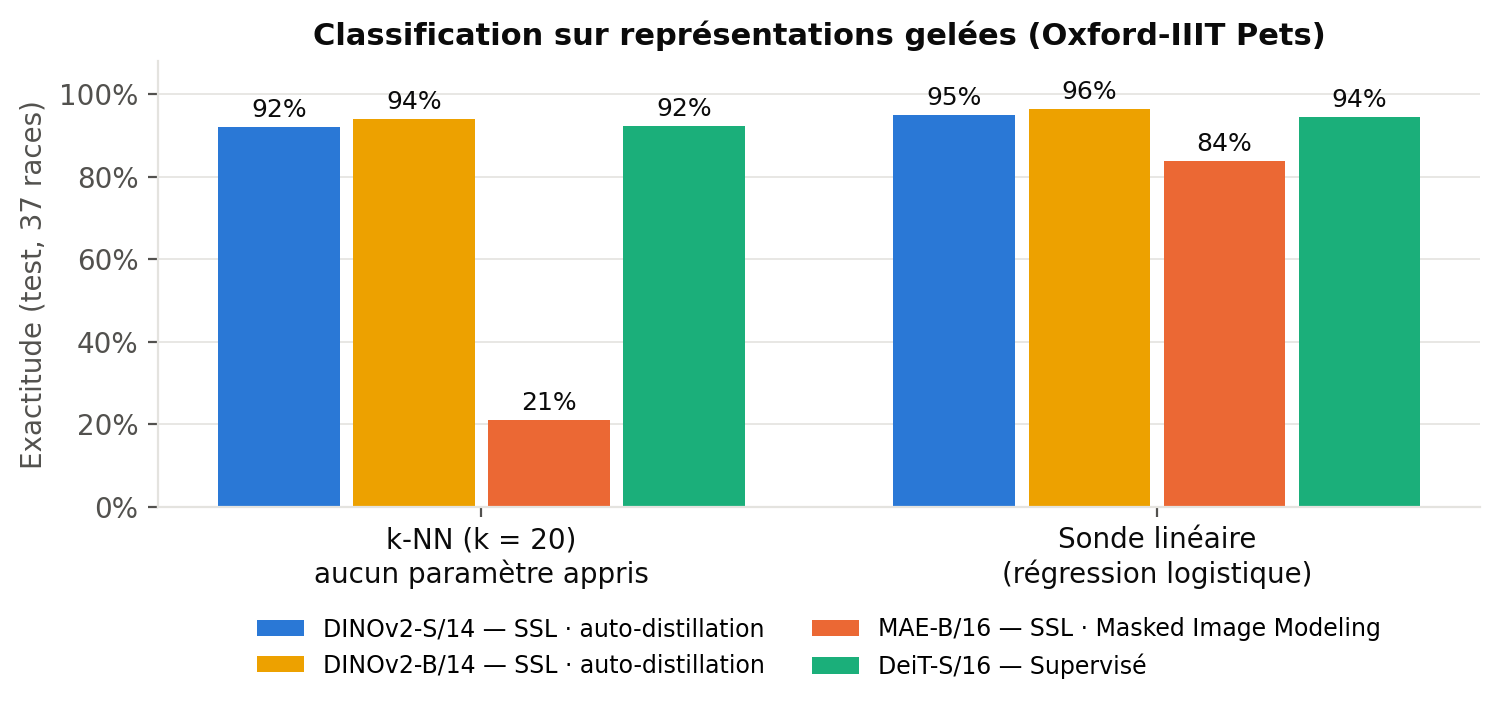
\includegraphics[width=\linewidth]{fig_accuracy.png}
    \caption{Exactitude k-NN et sonde linéaire.}\label{fig:acc}
  \end{subfigure}\hfill
  \begin{subfigure}[b]{0.46\textwidth}\centering
    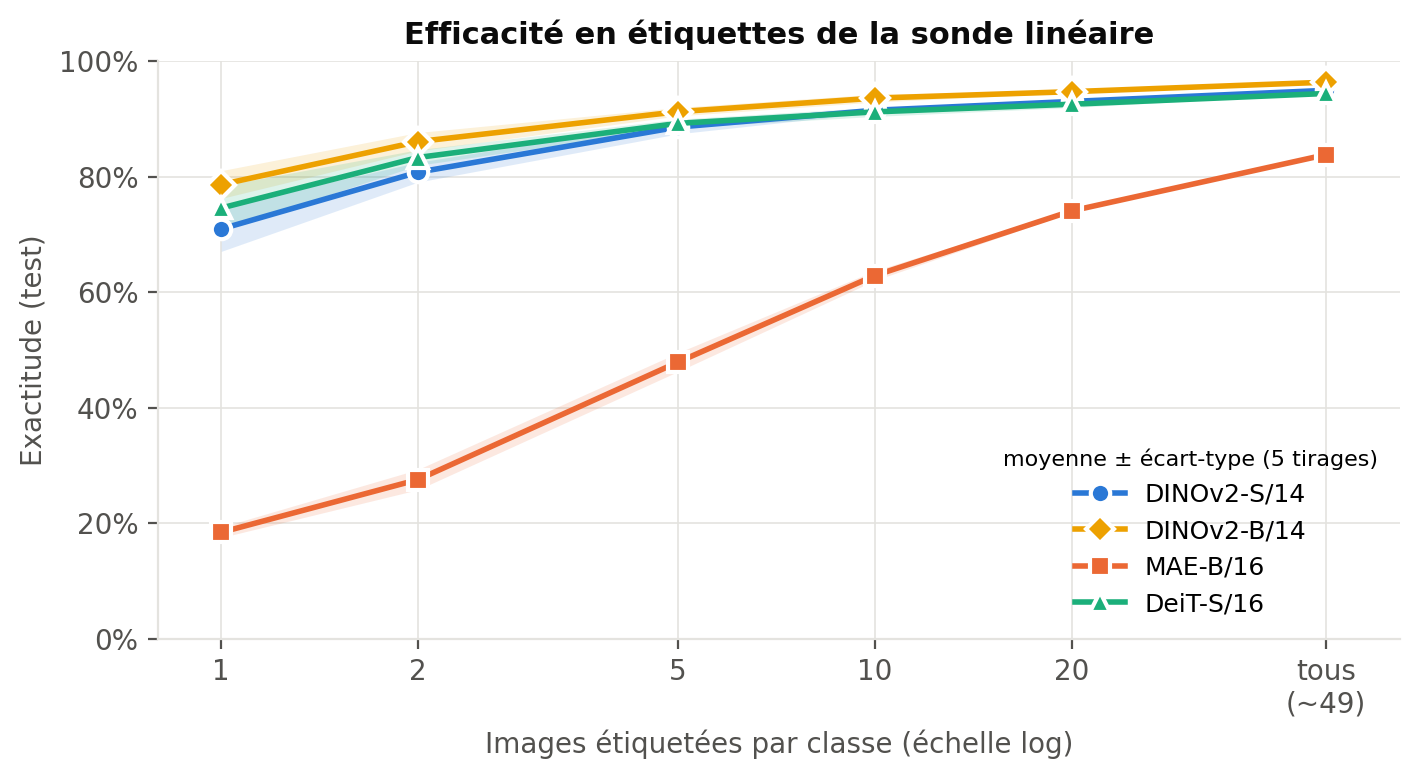
\includegraphics[width=\linewidth]{fig_label_efficiency.png}
    \caption{Efficacité en étiquettes.}\label{fig:eff}
  \end{subfigure}
  \caption{Classification sur représentations gelées (Oxford-IIIT Pets, 37 races).}
\end{figure}

\paragraph{Efficacité en étiquettes.} La figure~\ref{fig:eff} illustre l'argument central du SSL. Avec \textbf{une seule} image étiquetée par classe, DINOv2-B atteint \RSoneDinoB{} sur 37 races, contre \RSoneDeit{} pour DeiT-S, \RSoneDinoS{} pour DINOv2-S et \RSoneMae{} pour MAE. Avec 5 images par classe, il atteint \RSfiveDinoB{}. La connaissance utile se trouve déjà dans l'encodeur, et quelques exemples suffisent à la « lire ». MAE gelé, lui, a besoin de beaucoup plus d'exemples (\RSfiveMae{} avec 5 images par classe).

\paragraph{Recherche de similarité.} En recherche (figure~\ref{fig:retr}), la précision@5 vaut \RPfiveDinoB{} pour DINOv2-B, \RPfiveDinoS{} pour DINOv2-S, \RPfiveDeit{} pour DeiT-S et seulement \RPfiveMae{} pour MAE. Les erreurs de DINOv2 portent sur des races voisines (Bengal et Egyptian Mau, par exemple). Celles de MAE sont instructives : ses voisins partagent la couleur ou la pose de la requête plutôt que sa race, signe de features de plus bas niveau. Nous avons enfin testé deux requêtes absentes de la galerie et fortement transformées, construites à partir d'une image de race \RsearchTrue. La version recadrée, pivotée et en noir et blanc est correctement reconnue (\RsearchCrop, \RsearchCropConf{} des votes du k-NN). Le « croquis » obtenu par filtre de contours est en revanche classé \RsearchSketch : la robustesse aux changements de domaine extrêmes reste limitée.

\begin{figure}[ht]
  \centering
  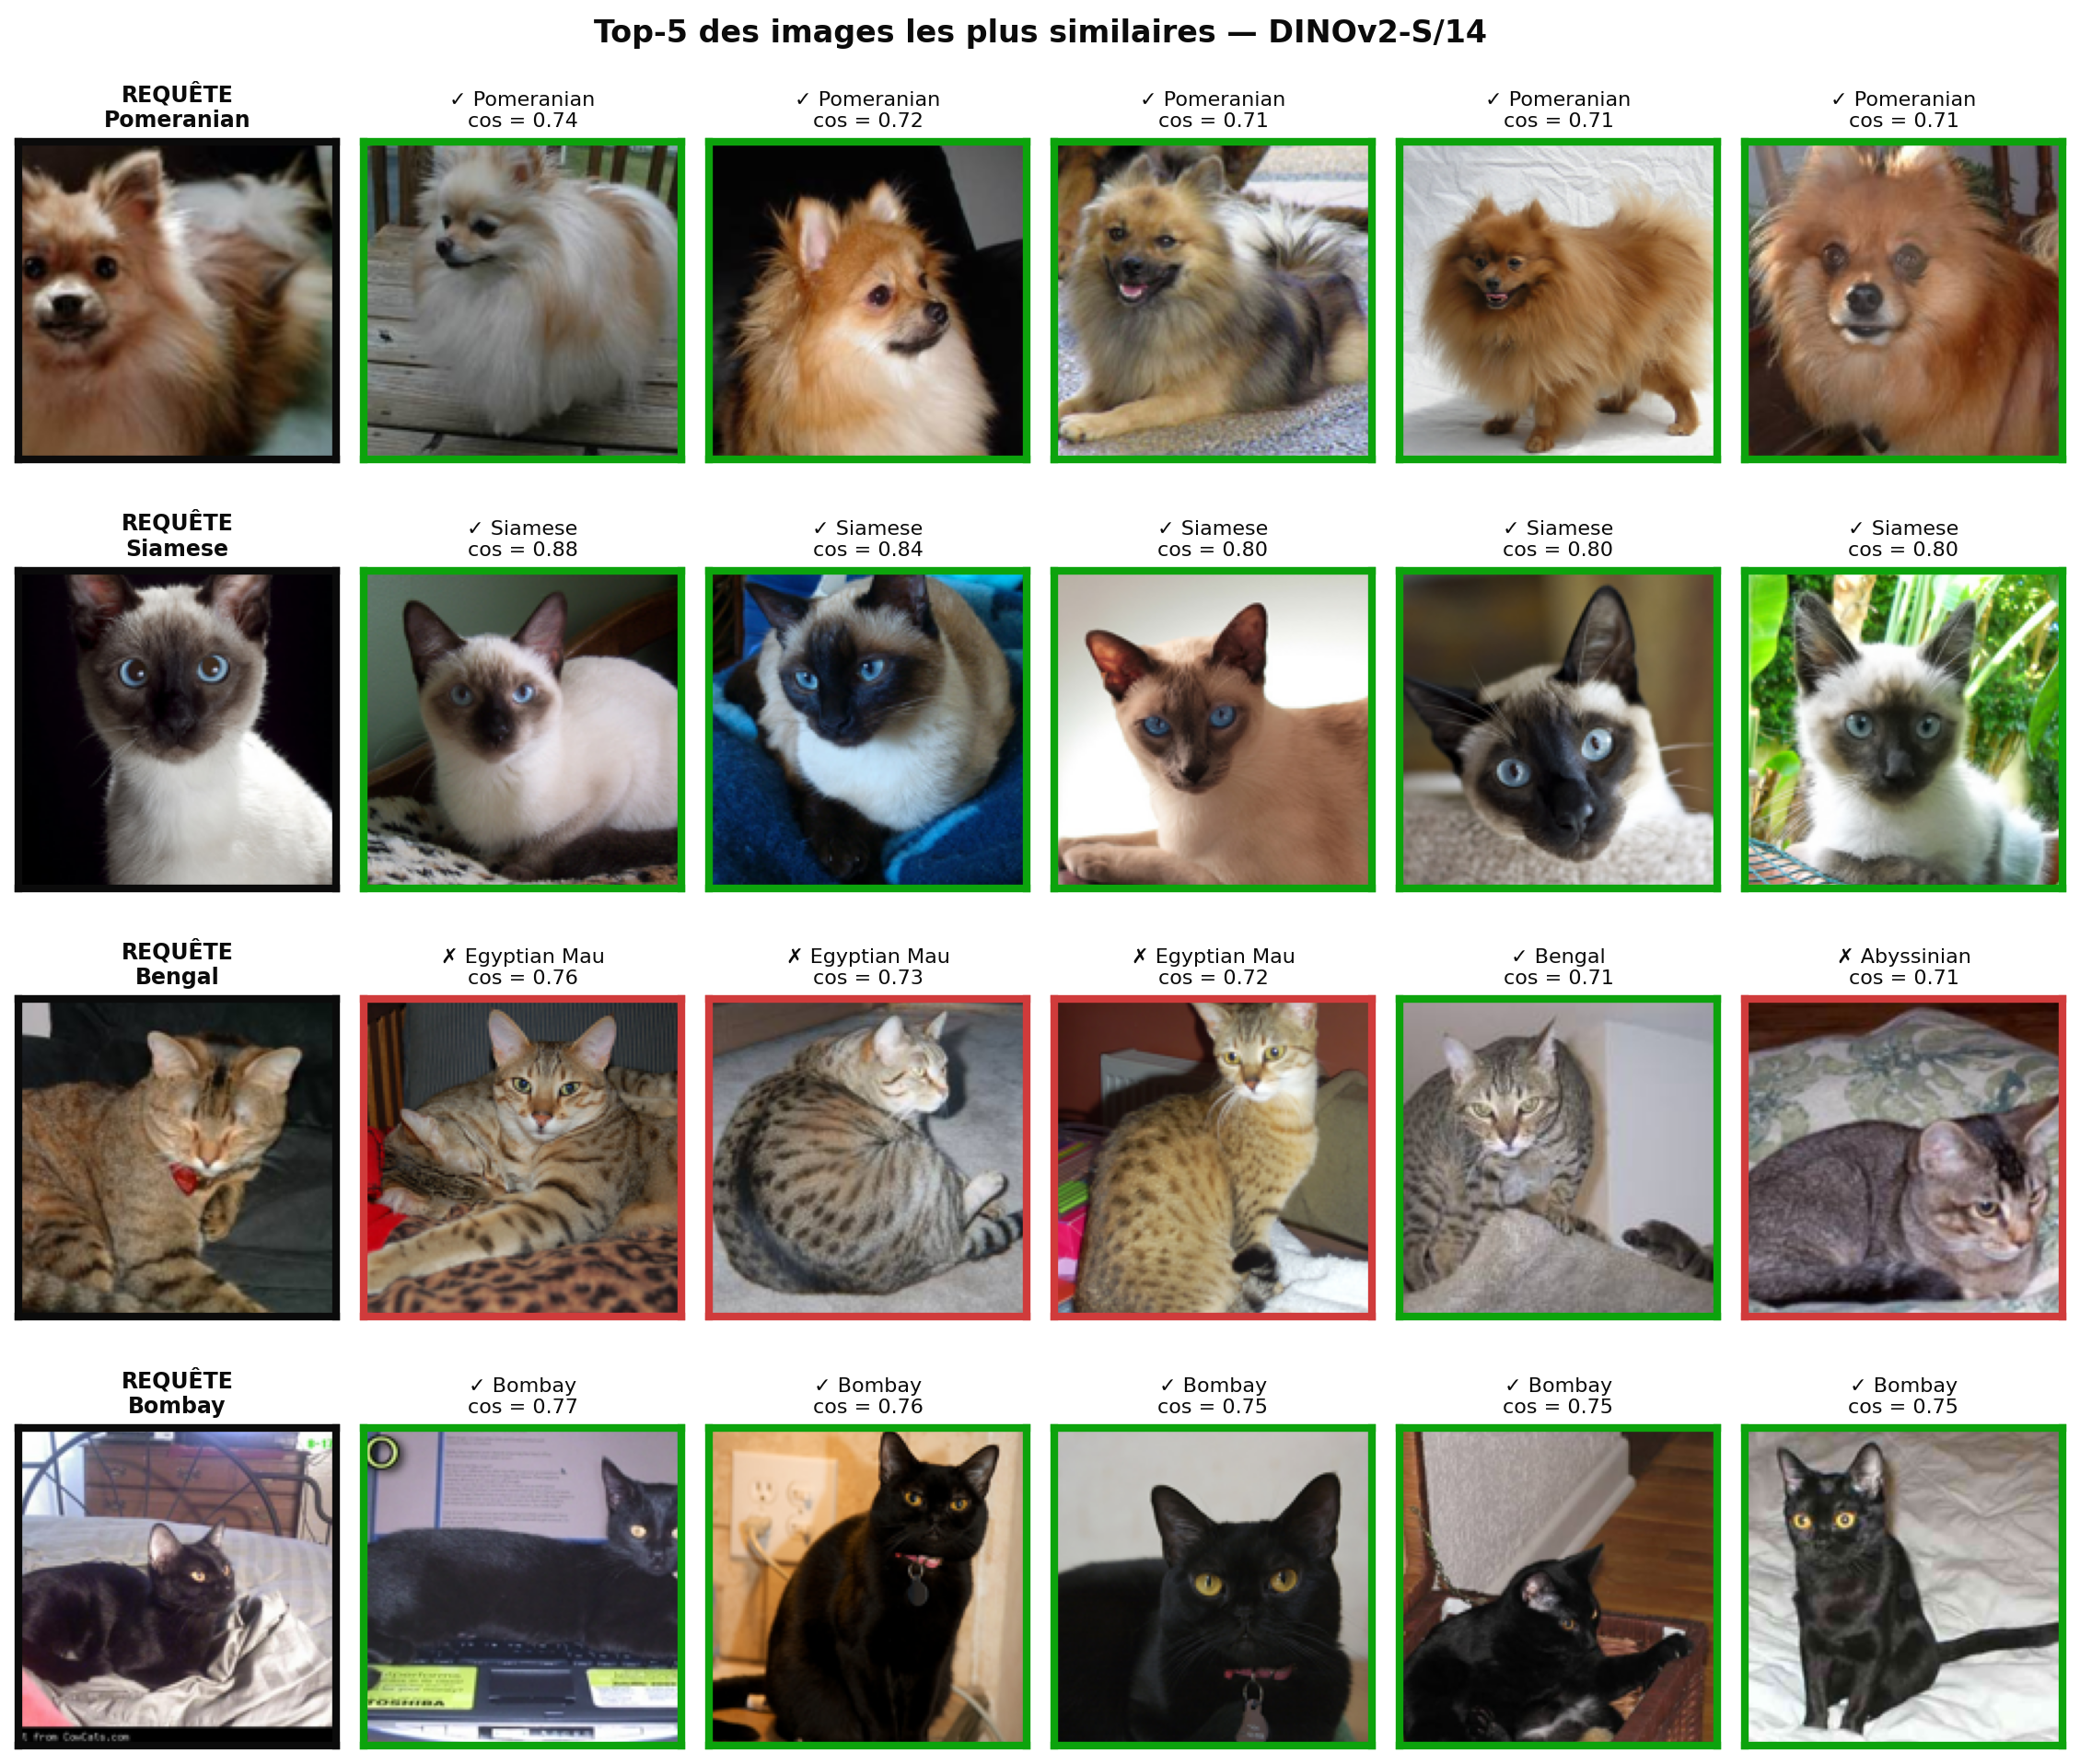
\includegraphics[width=0.78\textwidth]{fig_retrieval_dinov2.png}
  \caption{Recherche d'images similaires avec DINOv2-S/14 : chaque requête (à gauche) et ses 5 plus proches voisins dans la galerie (cadre vert : même race).}
  \label{fig:retr}
\end{figure}

\paragraph{Structure de l'espace et propriétés émergentes.} La projection t-SNE (figure~\ref{fig:tsne}) montre des groupes nets par race pour DINOv2 et DeiT-S, alors que MAE mélange toutes les races. Les scores de silhouette le confirment : \RSilDeit{} (DeiT-S), \RSilDinoB{} (DINOv2-B), \RSilDinoS{} (DINOv2-S) et \RSilMae{} (MAE). Que le supervisé soit le plus compact s'explique : il a été entraîné explicitement à séparer des classes ImageNet proches de celles de Pets. Enfin, une ACP sur les tokens de patches (figure~\ref{fig:pca}) sépare l'animal du fond sans aucune supervision dense, et ses composantes suivantes font apparaître des parties cohérentes (tête, corps) d'une image à l'autre. Mesurée avec les masques \emph{trimap} du jeu de données, l'IoU de ce masque non supervisé atteint \RIouDinoS{} pour DINOv2-S et \RIouDinoB{} pour DINOv2-B, contre \RIouDeit{} pour DeiT-S, dont les cartes sont plus bruitées. MAE (\RIouMae) ne fait pas mieux qu'un simple carré central (\RIouCenter).

\begin{figure}[ht]
  \centering
  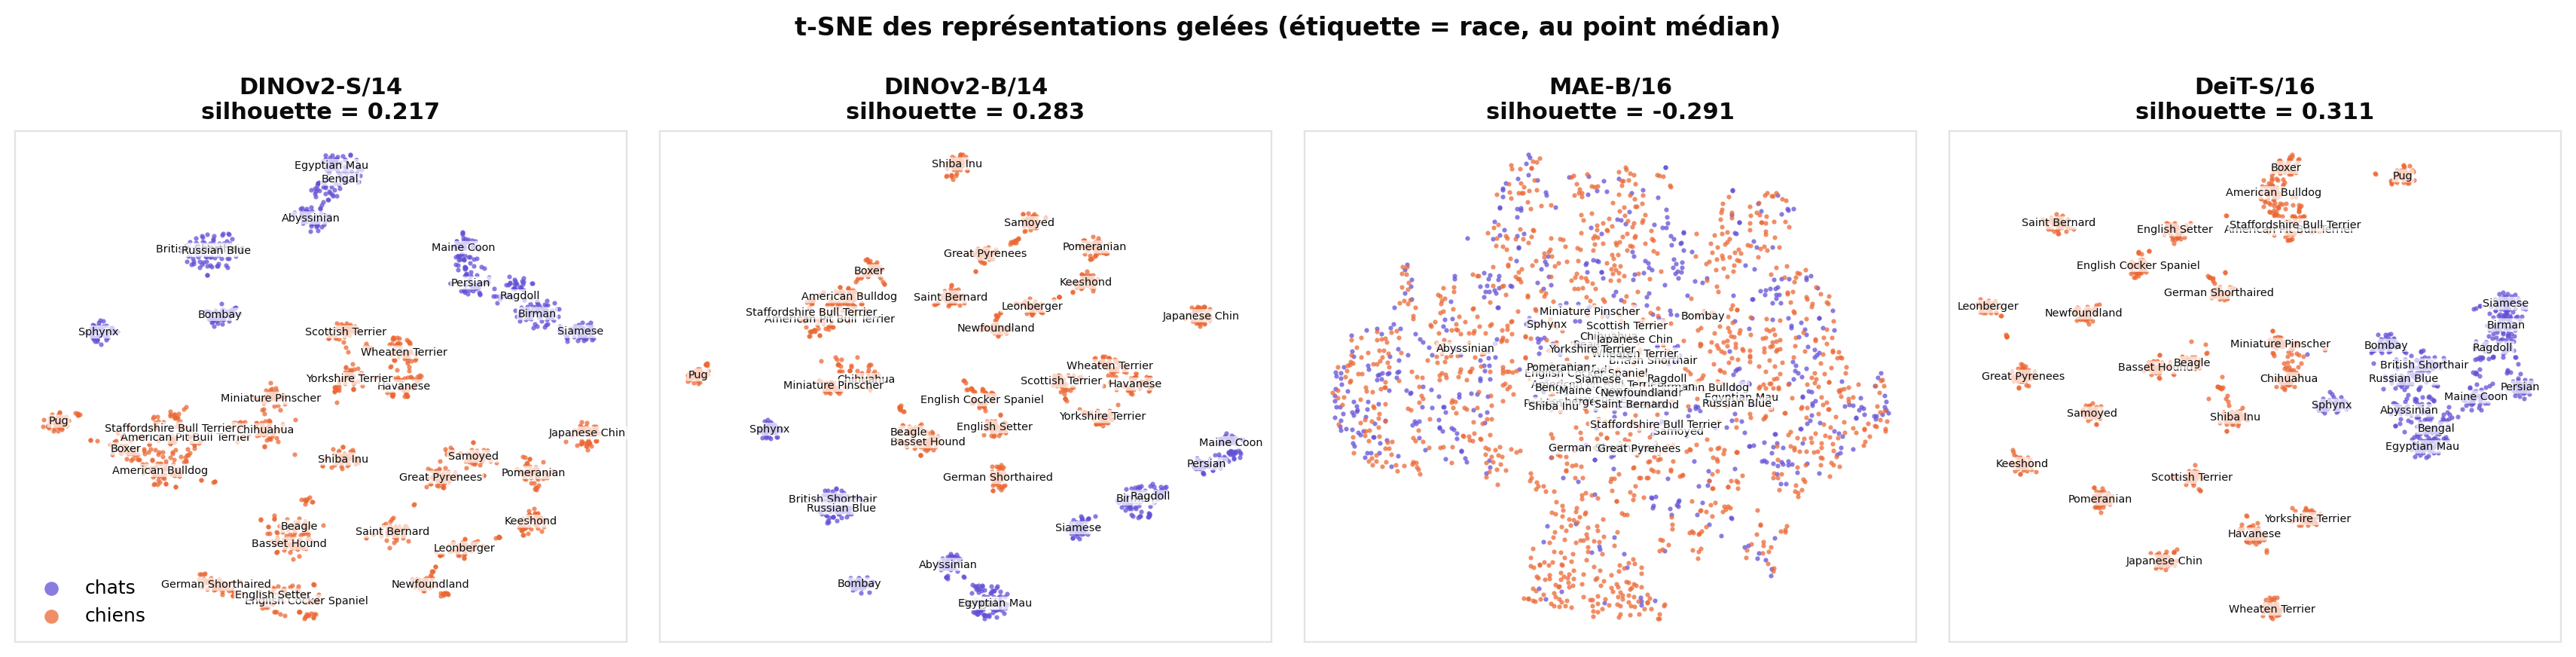
\includegraphics[width=\textwidth]{fig_tsne.png}
  \caption{t-SNE des représentations de test (couleur : espèce ; étiquette : race au point médian). Les races forment des groupes distincts pour DINOv2 et DeiT-S, et sont mélangées pour MAE.}
  \label{fig:tsne}
\end{figure}
\begin{figure}[ht]
  \centering
  \begin{subfigure}[b]{0.62\textwidth}\centering
    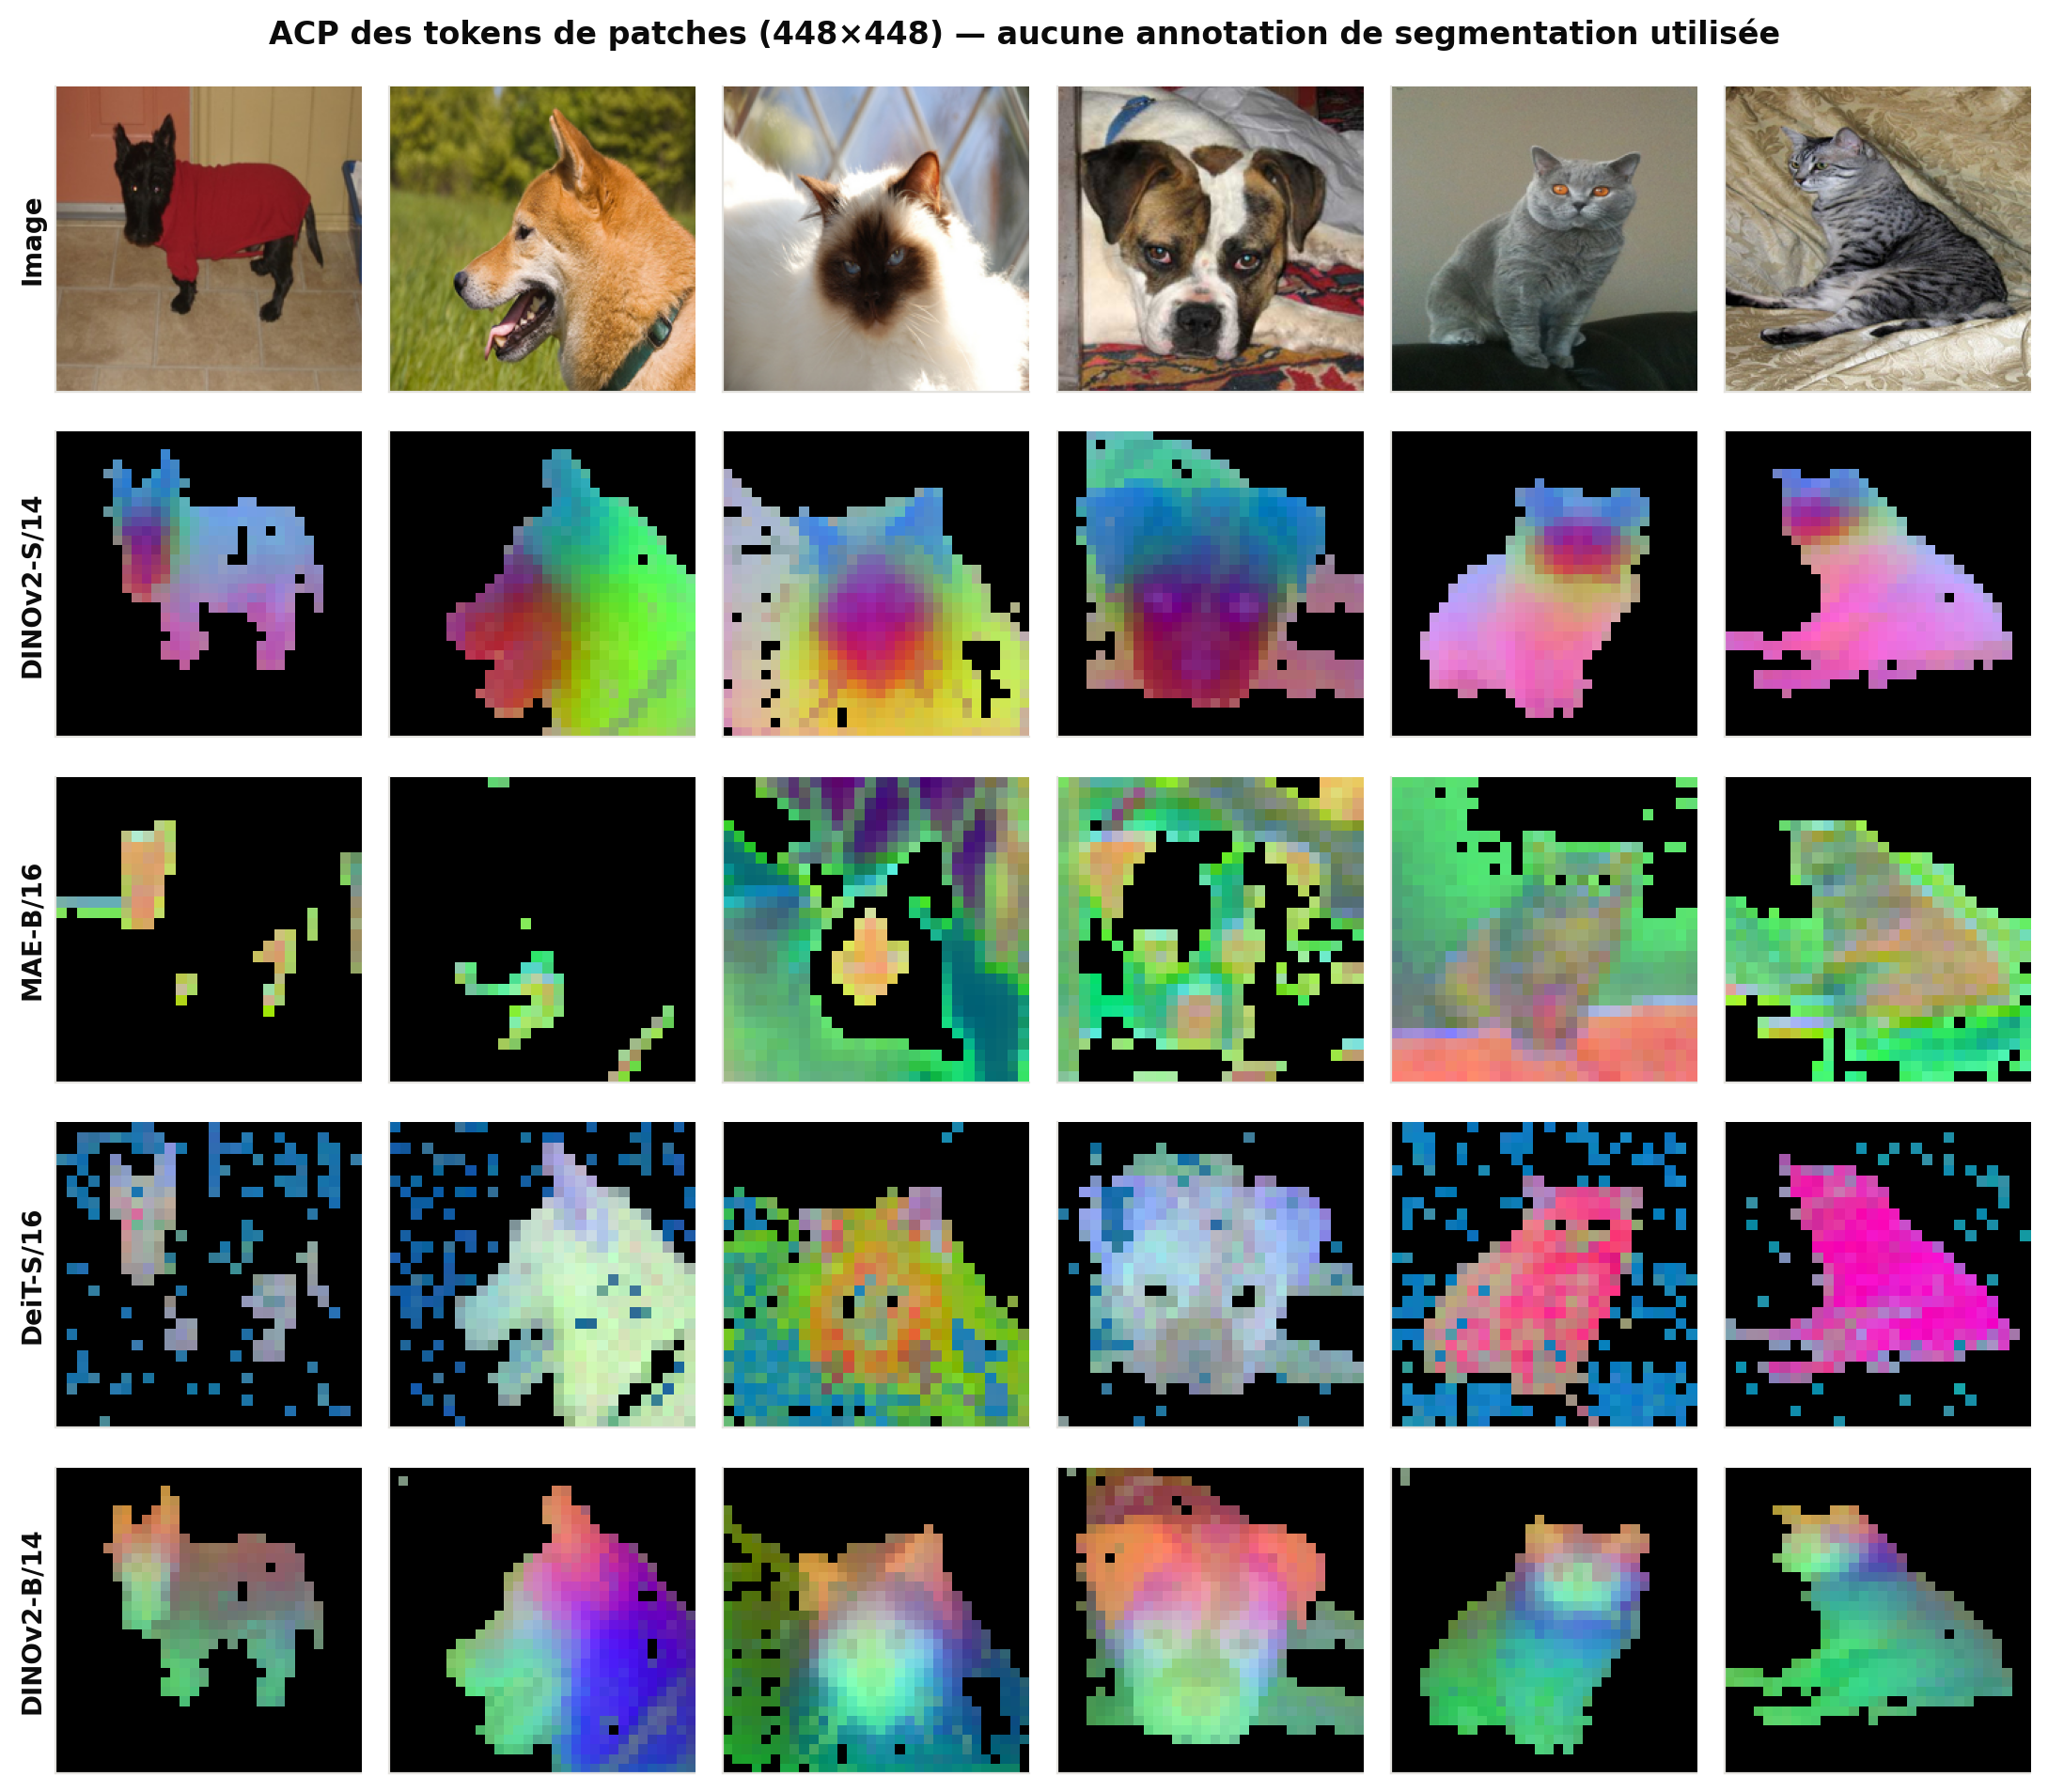
\includegraphics[width=\linewidth]{fig_pca_patches.png}\caption{ACP des tokens de patches (RVB = 3 composantes).}
  \end{subfigure}\hfill
  \begin{subfigure}[b]{0.36\textwidth}\centering
    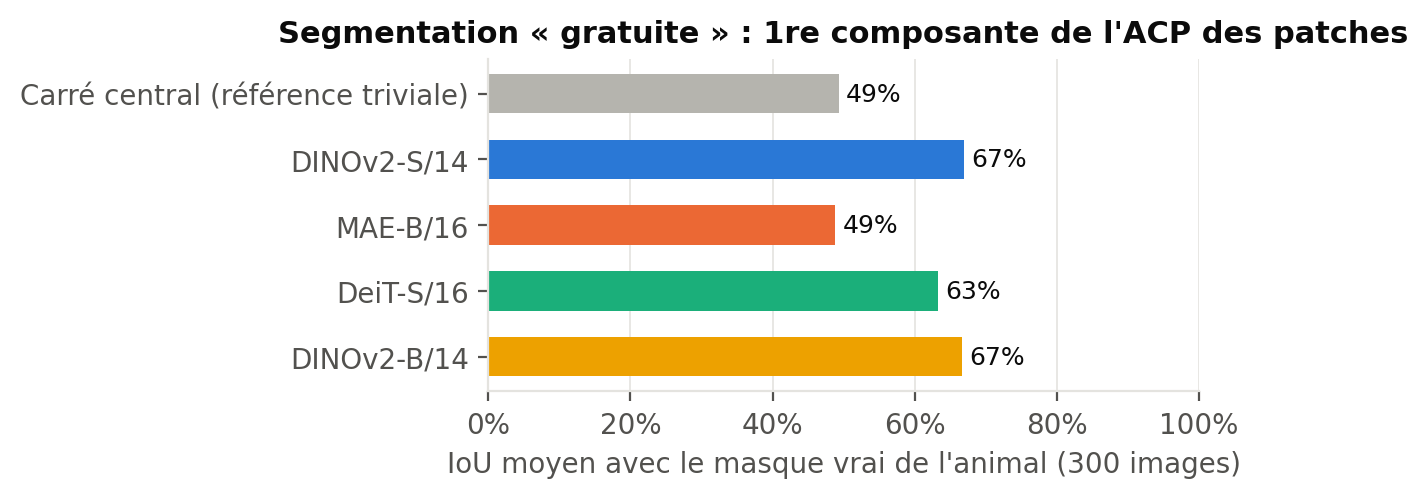
\includegraphics[width=\linewidth]{fig_seg_iou.png}\caption{IoU avec les masques vrais.}
  \end{subfigure}
  \caption{Segmentation émergente : les tokens de patches séparent l'animal du fond et ses parties sans annotation.}
  \label{fig:pca}
\end{figure}

% ======================================================================
\section{Comparaison et analyse critique}
\begin{table}[ht]
  \centering\small
  \caption{Comparaison des principales approches (sonde linéaire ImageNet-1k, valeurs publiées).}
  \label{tab:comp}
  \begin{tabularx}{\textwidth}{l l c c L L}
    \toprule
    Méthode & Signal & Négatifs & Linéaire & Point fort & Limite\\
    \midrule
    SimCLR & vues augmentées & oui & 69,3 (R50) & simplicité & très grands batchs\\
    MoCo v3 & vues augmentées & oui & 76,7 (ViT-B) & stable sur ViT & augmentations manuelles\\
    MAE & pixels masqués & non & 68,0 (ViT-B) & rapide ; meilleur en fine-tuning & features non linéaires\\
    DINO & vues multi-crop & non & 78,2 (ViT-B/16) & k-NN, attention & hyperparamètres sensibles\\
    DINOv2 & DINO + iBOT + KoLeo & non & 84,5 (ViT-B/14) & features gelées universelles & coût, curation\\
    CLIP & texte associé & oui & -- & zero-shot par le texte & détails visuels fins\\
    \bottomrule
  \end{tabularx}
\end{table}

\paragraph{Performances.} Le tableau~\ref{tab:comp} et nos expériences dessinent une hiérarchie cohérente. L'apprentissage contrastif apprend des invariances globales mais dépend des augmentations. Le masquage capture des détails locaux et excelle après fine-tuning (MAE : 87,8\,\% sur ImageNet avec un ViT-H$_{448}$, sans données externes), mais produit des features gelées médiocres. DINOv2 combine les objectifs global (DINO) et local (iBOT) à grande échelle et obtient des features directement exploitables, y compris pour des tâches denses.

\paragraph{Limites.} (i) \emph{Dépendance aux données} : la curation de DINOv2 utilise des jeux de référence (dont ImageNet) comme ancres, ce qui oriente la distribution apprise et peut transmettre des biais du web. (ii) \emph{Absence de langage} : contrairement à CLIP, DINOv2 ne permet pas de classification zero-shot par le texte. (iii) \emph{Artefacts} : des tokens de haute norme dans les cartes d'attention ont motivé l'ajout de registres. (iv) \emph{Évaluation} : la sonde linéaire ne mesure qu'une facette de la qualité ; MAE est faible selon ce critère mais excellent en transfert. Notre expérience a elle-même ses limites : un seul jeu de données, des budgets de pré-entraînement très inégaux (DINOv2-S est distillé d'un ViT-g entraîné sur 142 M d'images ; DeiT-S n'a vu qu'ImageNet-1k), et un recouvrement possible entre les races de Pets et les classes d'ImageNet.

\paragraph{Coûts.} Le pré-entraînement reste réservé à quelques acteurs : le ViT-g de DINOv2 a demandé 22\,016 heures de GPU A100, soit 9,7 MWh et 3,7 t CO$_2$eq. MAE réduit ce coût d'un facteur 3 grâce au masquage. En revanche, la réutilisation est très bon marché : toute notre démonstration tourne sur un GPU portable de 4 Go, à \RIpsDinoS{} images/s pour DINOv2-S, et l'extraction des features ne prend que quelques dizaines de secondes par modèle.

% ======================================================================
\section{Conclusion}
Les Vision Foundation Models déplacent l'effort de l'annotation vers le pré-entraînement : un encodeur est appris une fois, sans étiquettes, puis réutilisé partout avec peu de données. L'apprentissage auto-supervisé en est le moteur, à travers trois idées complémentaires : comparer des vues (contrastif), reconstruire l'image masquée (MAE) et s'auto-distiller (DINO). DINOv2 les réunit à grande échelle et produit des représentations gelées « universelles ». Notre expérience le confirme : sans aucun fine-tuning, DINOv2 permet une recherche de similarité et une classification de qualité. Il égale un modèle supervisé de même taille sans avoir vu d'étiquette et le dépasse dans sa version B, avec une forte efficacité en étiquettes et une segmentation émergente. Elle illustre aussi les limites des features MAE gelées et une robustesse imparfaite aux changements de domaine extrêmes. Plusieurs pistes prolongent ces travaux : DINOv3 (ViT de 7 milliards de paramètres, 1,7 milliard d'images et \emph{Gram anchoring} pour préserver les features denses~\citep{simeoni2025dinov3}), la prédiction dans l'espace latent (I-JEPA), et l'alignement avec le langage ou l'adaptation par prompts visuels.

\clearpage   % place tous les flottants (figures, tableaux) avant la bibliographie
\footnotesize
\setlength{\bibsep}{2pt}
\bibliographystyle{abbrvnat}
\bibliography{../references}

\end{document}
